\documentclass[11pt]{article}

\newcommand{\cnum}{CM146}
\newcommand{\ced}{Fall 2018}
\newcommand{\ctitle}[3]{\title{\vspace{-0.5in}\cnum, \ced\\Problem Set #1: #2}}
\usepackage{enumitem}
\newcommand{\solution}[1]{{{\color{black}{\bf Solution:} {#1}}}}
\usepackage[usenames,dvipsnames,svgnames,table,hyperref]{xcolor}
\usepackage{amsmath}
\usepackage{graphicx}
\usepackage[utf8x]{inputenc}
\usepackage{listings} %for listings of the source code


\renewcommand*{\theenumi}{\alph{enumi}}
\renewcommand*\labelenumi{(\theenumi)}
\renewcommand*{\theenumii}{\roman{enumii}}
\renewcommand*\labelenumii{\theenumii.}

\begin{document}
\ctitle{02}{Jonathan Chu}
\date{}
\maketitle
\vspace{-0.75in}

\section{(on CCLE)}
\section{(on CCLE)}

\section{Understanding Linear Separability}
\begin{enumerate}
\item %3a
\solution{
If $\delta$ = 0, we have:
$$y_i(\boldsymbol{w^Tx_i}+\theta) \geq 1$$
Trivially, this inequality holds when $sgn(y_i) = sgn(\boldsymbol{w^Tx_i}+\theta)$ and $|\boldsymbol{w^Tx_i}+\theta| \geq 1$.

The matching signs of $y_i$ and $\boldsymbol{w^Tx_i}$ indicate these values of $\boldsymbol{w}$ and $\theta$ satisfy equation (1). Therefore D is linearly separable.
}

\item %3b
\solution{
For $0 < \delta < 1$, it still holds that $sgn(y_i) = sgn(\boldsymbol{w^Tx_i}+\theta)$, meaning that D remains linearly separable, and $|\boldsymbol{w^Tx_i}+\theta| < 1$ for some i, which is not of any concern.

However, if the minimum $\delta \geq 1$, we have
$$y_i(\boldsymbol{w^Tx_i}+\theta) \geq c, \text{ } c \leq 0$$
and D is not linearly separable.
}

\item %3c
\solution{
The minimum value we can achieve for $\delta$ is 0. If this is the case, we seek $\boldsymbol{w}$ and $\boldsymbol{x}$ that satisfy the following:
$$y_i(\boldsymbol{w^Tx_i}+\theta) \geq 0$$
Trivially, $\boldsymbol{w} = \boldsymbol{0}$, $\theta = 0$ satisfy the above inequality yet clearly will not separate D.
}

\item %3d
\solution{
Trivially, we see that $\boldsymbol{w}=[1, 1, 1]$, $\theta=0$, $\delta=0$ is an optimal solution.

In fact, any solution with 
$$\delta = 0$$ 
$$|\boldsymbol{w^Tx_i}+\theta| = |w_1x_1 + w_2x_2 + w_3x_3 + \theta| \geq 1$$
$\implies |w_1 + w_2 + w_3 + \theta| \geq 1$ and $|-w_1 + -w_2 + -w_3 + \theta| \geq 1$

is optimal.
}
\end{enumerate}

\section{Implementation: Polynomial Regression}
\begin{enumerate}
\item %4a
By inspection, linear regression would not model the data very accurately. Although lines with negative slope on both the training and test data seem like they would perform moderately well, there would still be high training and test error, since the square distance from points to the line would be somewhat large for many of the data points. 


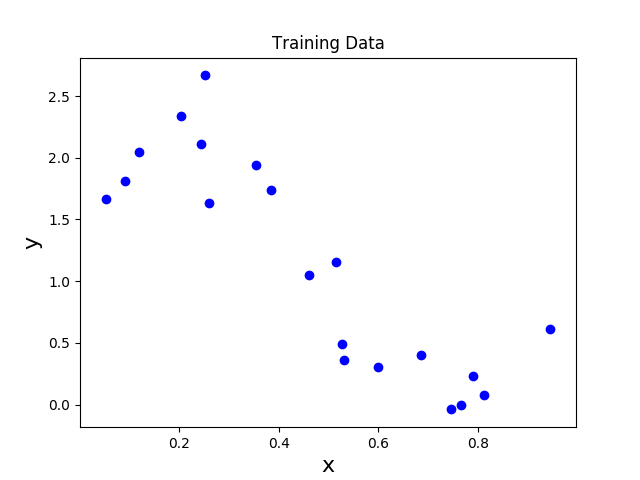
\includegraphics[width=\linewidth]{Training_Data.png}
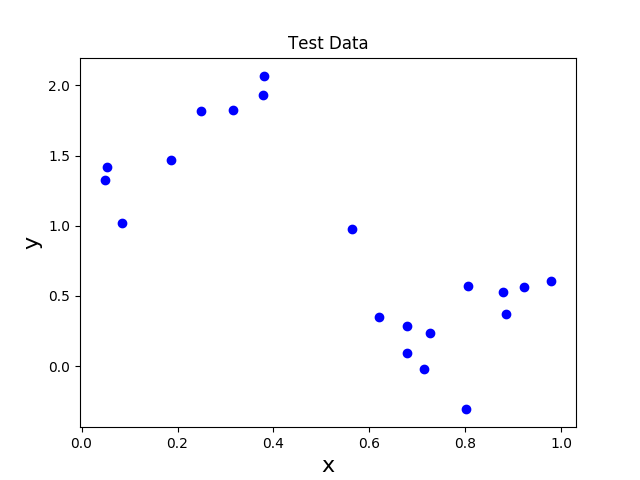
\includegraphics[width=\linewidth]{Test_Data.png}

\item %4b
\begin{lstlisting}
Phi = np.concatenate((np.ones(np.shape(X)), X), 1)
\end{lstlisting}

\item %4c
\begin{lstlisting}
y = np.dot(self.coef_, np.transpose(X))
\end{lstlisting}

\item %4d
Investigating linear regression...

	 --The model cost with zero weights is 40.233847


\begin{center}
\begin{tabular}{ |c|c|c|c| } 
 \hline
 $\eta$ & $\#$ Iterations & Final Coefficients & Final Value of J($\theta$)\\ 
 \hline
 0.00407 & 10000 & -9.40470 x $10^{18}$, -4.65229 x $10^{18}$ & 1.35545 x $10^{38}$ \\ 
 0.001 & 764 & & 0.195629 \\ 
 0.0001 & 7020 & & 0.195629 \\ 
 0.00001 & 10000 & & 0.204320 \\ 
 \hline
\end{tabular}
\end{center}



\end{enumerate}

\end{document}
